
\documentclass[a4paper,12pt]{article}

\usepackage[a4paper, total={6in, 8in}, left=30mm]{geometry}
\usepackage{pdfpages}

\usepackage{cmap}
\usepackage[T2A]{fontenc}
\usepackage[utf8]{inputenc}
\usepackage[english,russian]{babel}
\usepackage{fancyhdr}
\usepackage{minted}
\usepackage{hyperref}
\usepackage{amsmath}
\usepackage{graphicx}
\usepackage[document]{ragged2e}

\providecommand{\tightlist}{%
  \setlength{\itemsep}{0pt}\setlength{\parskip}{0pt}}

\hypersetup{
  pdfborderstyle={/S/U/W 1}
}

\graphicspath{{./images/}}

\pagestyle{fancy}
\fancyhf{}
\lhead{Антон Завьялов, ПИ-72}
\rhead{\textbf{Лабораторная №2}}
\cfoot{\thepage}

\makeatletter
\def\@seccntformat#1{%
  \expandafter\ifx\csname c@#1\endcsname\c@section\else
  \csname the#1\endcsname\quad
  \fi}
\makeatother

\begin{document}
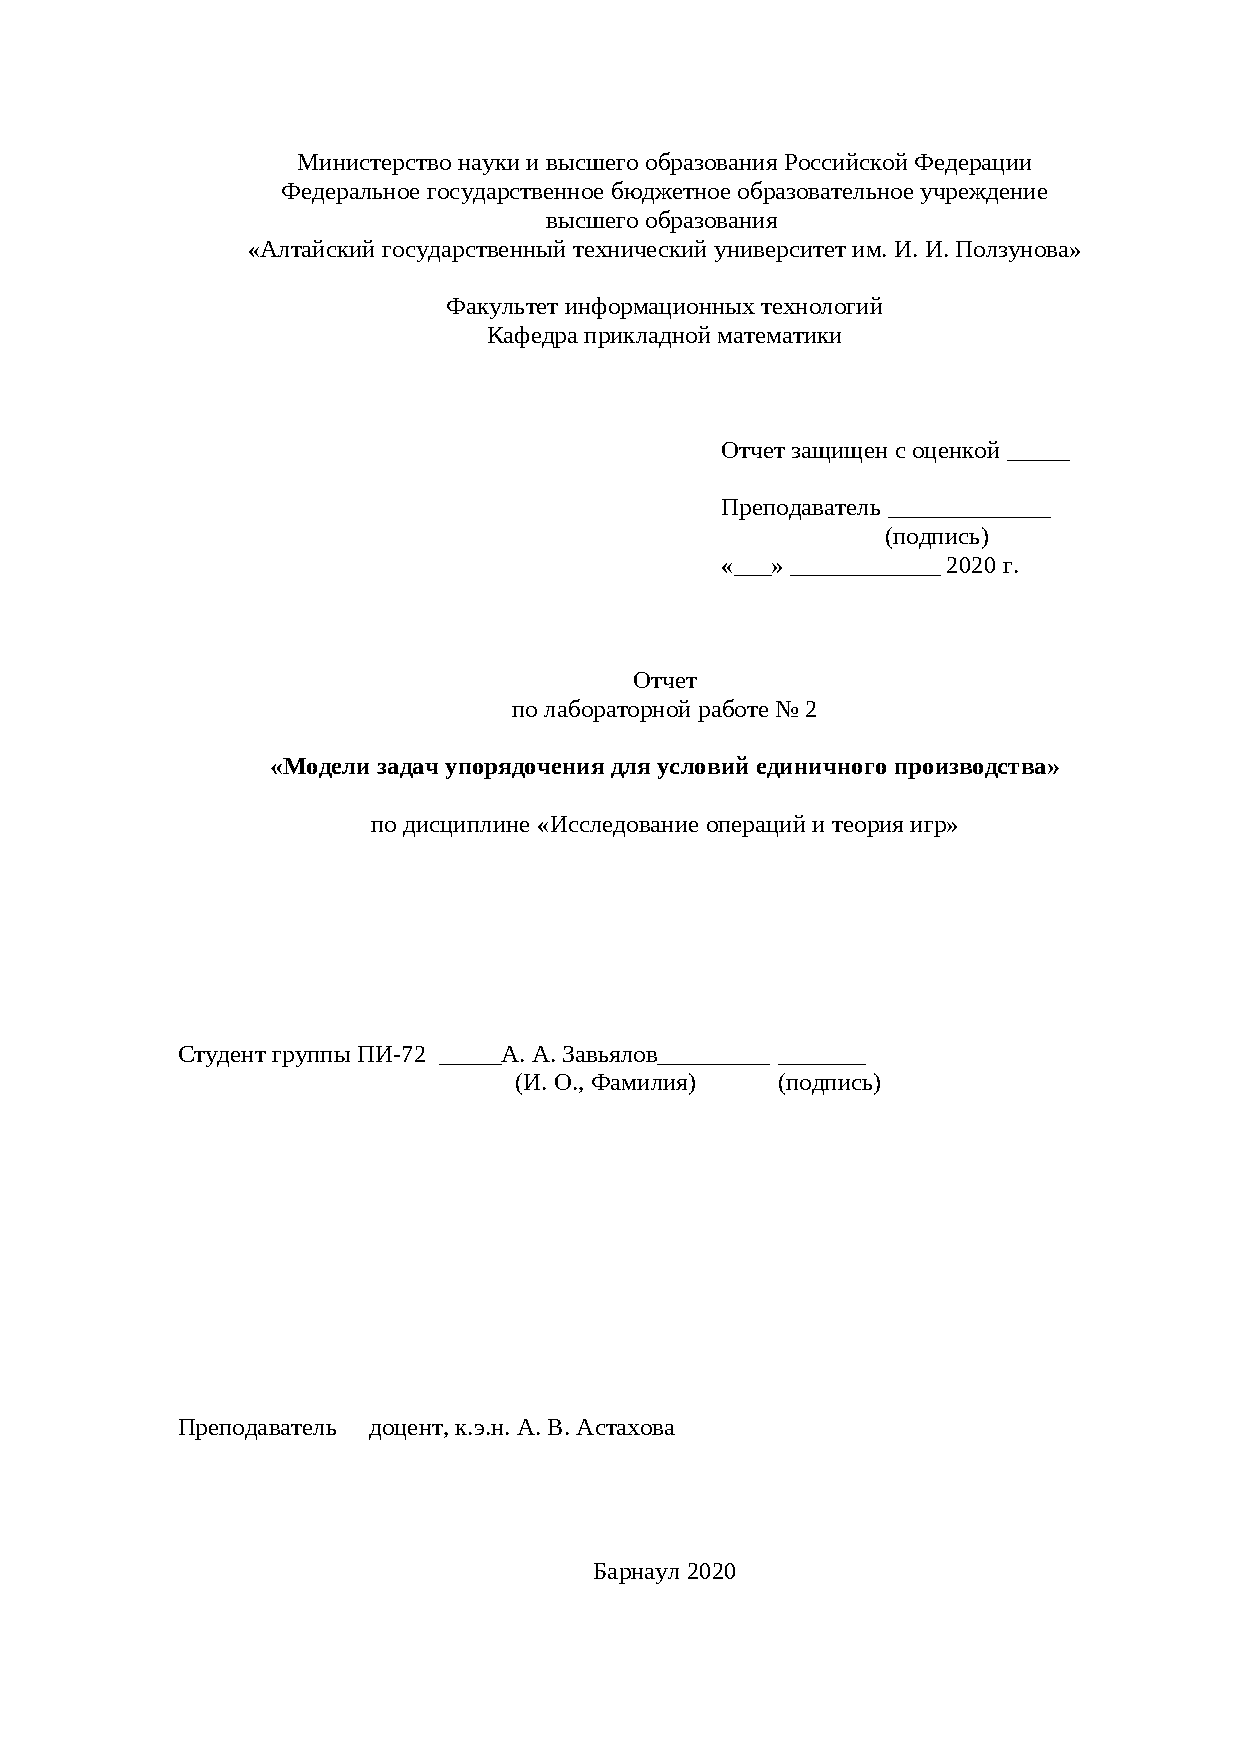
\includepdf[pages={1}]{title.pdf}

\section{\normalsize{Задание на лабораторную работу}}
\begin{flushleft}
\textbf{Задание 1. Построение графика Ганта для учебного примера Фишера
-Томпсона}
\justify
\begin{enumerate}
\item
  Ознакомиться с теоретическими основами решения задач теории расписаний
  для условий единичного производства, используя методические указания
  по теме. См. файл Module\_1\_Modeli\_zadach\_uporyadocheniya (в
  системе Илиас), пункт «Задачи упорядочения n$\times$m».
\item
  С помощью компьютерной программы Models или вручную на листе клетчатой
  бумаги, используя эвристический алгоритм запуска деталей в обработку,
  построить вариант графика Ганта загрузки 6 станков ($A$, $B$, $C$, $D$, $E$, $F$),
  являющийся технологически допустимым и отвечающим заданному
  ограничению по времени обработки всех 6 деталей \textbf{Т $\le$ 68} (ед.
  времени). Исходные данные для решения задачи заданы в двух таблицах $F$
  и $T$ на рис. 1. Номера строк обеих таблиц i -- соответствуют индексам
  (номерам) деталей; номера столбцов j -- соответствуют номерам
  технологических операций по маршруту. Значения элементов матриц F и Т
  соответственно: f\textsubscript{ij} -- шифр станка, на котором
  выполняется операция j делали i;\\
  t\textsubscript{ij}-- норма времени этой операции на данном станке. 

  Очевидно, что технологический маршрут по операциям детали i отображен в
  строке i матрицы F. Например, деталь № 2 при ее производстве проходит
  последовательно через обработку на станках В, C, E, F, А, D. Иная
  последовательность обработки, естественно, не допустима.

  При этом если, например, f\textsubscript{23 }= Е, то операция № 3 для
  детали № 2 выполняется на станке Е. Норма времени для нее
  t\textsubscript{23}= 10 (ед. времени) записана в матрице Т (нормы
  времени по операциям).

\item
  Определить следующие параметры построенного графика загрузки станков:

\begin{itemize}
\item
  длительность производственного цикла обработки всех деталей на всех
  станках;
\item
  время простоя каждого станка;
\item
  время «пролеживания» деталей в ожидании обработки на каждом станке. 
\begin{flushleft}\end{flushleft}
\begin{figure}
    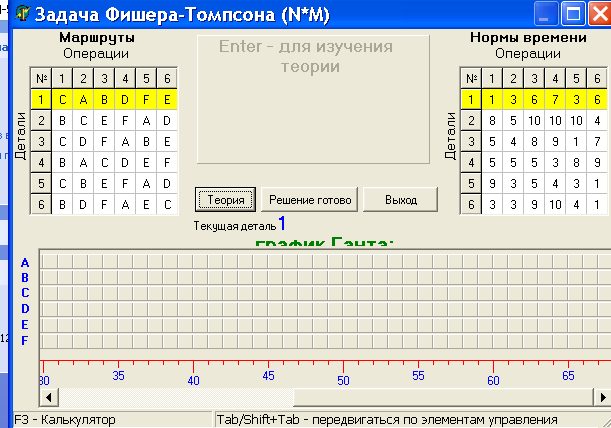
\includegraphics[width=8.832cm,height=6.156cm]{pic_1.png}
    \centering
    \caption{\small{Экранная форма при работе в пункте меню «Задача
    Фишера-Томпсона»}}
\end{figure}
\end{itemize}
\end{enumerate}
\raggedright
\textbf{Задание 2. Разработка алгоритма и программы имитационного
моделирования загрузки оборудования }
\justify
\begin{enumerate}
\item
  В соответствие с теоретическими основами решения задач теории
  расписаний для условий единичного производства (см. в Илиас параграф
  «Задачи упорядочения n$\times$m» в файле:
  Module\_1\_Modeli\_zadach\_uporyadocheniya), разработать алгоритм
  моделирования загрузки оборудования, взяв за основу принцип
  моделирования «по особым состояниям». 

  В алгоритме учесть процедуру упорядочения деталей в очереди с учетом
  выбора одного из двух заданных привила предпочтения запуска деталей в
  обработку -- в момент, когда у станка возникает очередь деталей.

  Вариант правил предпочтения, используемых при возникновении очереди
  деталей перед станком, задается преподавателем (см. файл «Правила
  предпочтения»).

\item
  Составить и отладить программу на алгоритмическом языке (по выбору
  студента), одна из процедур которой выбирает деталь из очереди у
  станка (\emph{если} очередь образовалась) по заданному правилу
  предпочтения. На вход программы подается информация о размерности двух
  матриц F и Т, описанных выше; содержание матриц (возможны маршруты
  различной длины); «номер» правила предпочтения (для вызова
  соответствующей процедуры упорядочения). Длины технологических
  маршрутов деталей могут быть разными. В результате моделирования
  необходимо рассчитать три параметра (выбранные в качестве показателей
  эффективности) построенного графика загрузки станков:

  \begin{itemize}
  \item
    длительность производственного цикла Т обработки всех деталей на всех
    станках;
  \item
    время простоя каждого станка;
  \item
    время «пролеживания» деталей в ожидании обработки на каждом станке. 
  \end{itemize}

  Требование к интерфейсу программы: результатом работы программы должен
  быть график Ганта, выведенный на экран монитора компьютера (в форме
  линейной диаграммы), три параметры, его характеризующие; линейные
  диаграмма, моделирующие очереди деталей перед станками, возникающие в
  процессе моделирования (также выведенные на экран).

\item
  Запустив программу два раза (на одних и тех же исходных данных) с
  двумя различными правилами предпочтения, и получив два варианта
  загрузки станков, проанализировать полученные показатели эффективности
  модели. Сделать вывод, каким образом и почему (в Вашем конкретном
  случае) правило предпочтения влияет на показатели эффективности
  графика загрузки оборудования. 
\end{enumerate}
\end{flushleft}

\pagebreak

\section{\normalsize{Выполнение работы}}
\begin{flushleft}
  \justify
  \begin{enumerate}
    \item Построен вариант графика Ганта загрузки 6 станков ($A, B, C, D, E, F$), являющийся технологически допустимым и отвечающим заданному ограничению по времени обработки всех 6 деталей \textbf{T $\le$ 68} (ед. времени):
    \begin{figure}[H]
      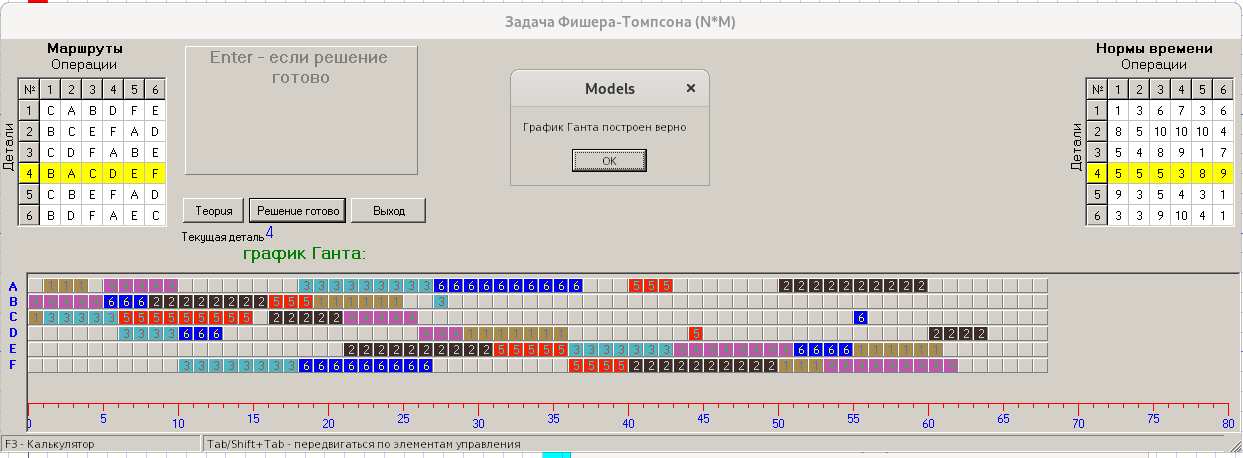
\includegraphics[width=15.25cm,height=6.5cm]{heuristics.png}
      \centering
      \caption{\small{График Ганта загрузки станков $A, B, C, D, E, F$}}
  \end{figure}
    \item Параметры графика загрузки станков:
    \begin{itemize}
      \item Длительность производственного цикла обработки всех деталей на всех станках: 64 (ед. времени);
      \item Время простоя каждого станка (ед. вр.):\newline A = 24, B = 38, C = 38, D = 42, E = 24, F = 43;
      \item Время «пролеживания» деталей в ожидании обработки на каждом станке (ед. вр.):\newline дет. 1 = 35, дет. 2 = 17, дет. 3 = 8, дет. 4 = 27, дет. 5 = 20, дет. 6 = 26.
    \end{itemize}
  \end{enumerate}
\end{flushleft}

\end{document}
